%%%%%%%%%%%%%%%%%%%%%%%%%%%%%%%%%%%%%%%%%
% Cleese Assignment (For Students)
% LaTeX Template
% Version 2.0 (27/5/2018)
%
% This template originates from:
% http://www.LaTeXTemplates.com
%
% Author:
% Vel (vel@LaTeXTemplates.com)
%
% License:
% CC BY-NC-SA 3.0 (http://creativecommons.org/licenses/by-nc-sa/3.0/)
% 
%%%%%%%%%%%%%%%%%%%%%%%%%%%%%%%%%%%%%%%%%

%----------------------------------------------------------------------------------------
%	PACKAGES AND OTHER DOCUMENT CONFIGURATIONS
%----------------------------------------------------------------------------------------

\documentclass[10pt]{article}
\input{activite.sty} % Include the file specifying the document structure and custom commands
\usepackage{subfig, dblfloatfix} % fix for bottom-placement of figure


\newtcolorbox{mybox}[1][]{
    colbacktitle=blue!10!white,
    colback=red!10!white,
    coltitle=blue!70!black,
    adjusted title={#1},
    fonttitle=\bfseries,
	% noattach
    % attach title to upper={\ --- \ }
    }



% \usepackage{activite}
%----------------------------------------------------------------------------------------
%	ASSIGNMENT INFORMATION
%----------------------------------------------------------------------------------------

% Required
\newcommand{\assignmentQuestionName}{Question} % The word to be used as a prefix to question numbers; example alternatives: Problem, Exercise
\newcommand{\assignmentClass}{Physique Chimie} % Course/class
\newcommand{\assignmentTitle}{Activité n°2} % Assignment title or name
\newcommand{\assignmentAuthorName}{Chapitre 2} %

%----------------------------------------------------------------------------------------
%	VARIABLES
%----------------------------------------------------------------------------------------

\newcommand{\titreActivite}{Activité 2: Le sens du courant} % titre de l'activité
\newcommand{\objectif}{ 	
	
	\begin{itemize}
		\item Comprendre l'effet du sens du courant sur le fonctionnement de certains dipôles.
		\item Comprendre le fonctionnement des diodes.
	\end{itemize}
}

\newcommand{\resumeContexte}{
	Le sens du courant a-t-il un effet sur certains dipôles ?
	} % titre de l'activité




%----------------------------------------------------------------------------------------

\begin{document}
%----------------------------------------------------------------------------------------
%	TITLE PAGE
%----------------------------------------------------------------------------------------
\date{}
\title{\titreActivite}
\maketitle % Print the title page

%----------------------------------------------------------------------------------------
%	QUESTION 1
%----------------------------------------------------------------------------------------

\underline{\textbf{Objectif}} :  \vspace{2pt}
\objectif

\vspace{4pt}

% \underline{\textbf{Contexte}} :  \textit{\contexte}

% \begin{center}
% 	\includegraphics[width=0.55\columnwidth]{activité.jpg} % Example image
% \end{center}
\textbf{\resumeContexte}
%%%%%%%%%%%%%%%%%%%%%%%%%%%%%%%%%%%%%%%%%%%%


\vspace{-12pt}
%% ----------------------------------

\assignmentSection{Votre mission travail}

\textbf{\underline{Matériel}} : Un pile, une lampe, des fils de connexion, un moteur, une DEL, deux pinces
 crocodile, un
interrupteur.

%----------------------------------------------------------------------------------------
%	QUESTION 1
%----------------------------------------------------------------------------------------
% \vspace{-10pt}

\begin{mybox}[Convention]
	(Une convention est un choix arbitraire
	, comme de rouler à droite pour les automobilistes en France). 
	
	Par convention,
	\textbf{le courant électrique circule de la borne +
	vers la borne –} à l’extérieur du générateur.
	On le représente par \textbf{l’extrémité d’une flèche} sur un schéma.

\end{mybox}

\begin{question}
	
	\questiontext{
	 \textbf{Compléter} les schémas suivants pour 
	 indiquer le sens du courant.
	}
	\end{question}
	
	\begin{center}
		\begin{minipage}[c]{0.45\textwidth}
			\centering
			\includegraphics[width=3.5cm]{lamp_lamp_inverted.png}
		\end{minipage}
		\hspace{0pt}
		\begin{minipage}[c]{0.45\textwidth}
			\centering
			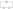
\includegraphics[width=3.5cm]{lamp_lamp.png}
		\end{minipage}
	\end{center}






%----------------------------------------------------------------------------------------
%	QUESTION 2
%----------------------------------------------------------------------------------------

\begin{question}
	\questiontext{
		Effet sur la lampe.
	}
	\end{question}


	\begin{minipage}[c]{0.55\textwidth}
		\subquestion{
			\textbf{Indiquer} le sens du courant sur chacun
		des schémas ci dessous.
		}

		\subquestion{
			\textbf{Réaliser} les circuits}	
			
		\subquestion{
			\textbf{Indiquer} l'état de la lampe 
			sur les pointillés.
			}
		\subquestion{
			\textbf{Écrire} une phrase de conclusion.
			}
	\end{minipage}
	\hspace{10pt}
	\begin{minipage}[c]{0.45\textwidth}
		\begin{minipage}[t]{0.45\textwidth}
			\includegraphics[width=4cm]{example-image}
		\end{minipage}
		\hspace{ 20pt}
		\begin{minipage}[t]{0.45\textwidth}
			\includegraphics[width=4cm]{example-image}
		\end{minipage}	
	\end{minipage}

	\vspace{10pt}

	\answerbox{3}

	

	%----------------------------------------------------------------------------------------
	%	QUESTION 3
	%----------------------------------------------------------------------------------------
	
	\begin{question}
		\questiontext{
		Effet sur le moteur.		
		}
		\end{question}

		\begin{minipage}[c]{0.65\textwidth}
			\subquestion{
				\textbf{Indiquer} le sens du courant sur chacun
			des schémas à droite.
			}
			\subquestion{
				\textbf{Réaliser} les circuits.
				}	
				
			\subquestion{
				\textbf{Indiquer} le sens de rotation du moteur sur les pointillés.
				}
	
			\subquestion{
				\textbf{Écrire} une phrase de conclusion.
				}
		\end{minipage}
		\hspace{0pt}
		\begin{minipage}[c]{0.25\textwidth}
			\begin{center}
				\includegraphics[width=4cm]{example-image}
			\end{center}
		\end{minipage}

		\vspace{10pt}
		\answerbox{3}

	%----------------------------------------------------------------------------------------
	%	QUESTION 4
	%----------------------------------------------------------------------------------------
	
	\begin{question}
		\questiontext{
		Effet sur la DEL.		
		}
		\end{question}

		\begin{minipage}[c]{0.65\textwidth}
					\subquestion{
					\textbf{Indiquer} le sens du courant sur chacun
				des schémas ci dessous.}
				\subquestion{
					\textbf{Réaliser} les circuits.
					}	
					
				\subquestion{
					\textbf{Indiquer} l'état de la DEL sur les pointillés.
					}
				\subquestion{
					\textbf{Écrire} une phrase de conclusion.
					}
		\end{minipage}
		\hspace{10pt}
		\begin{minipage}[c]{0.25\textwidth}
			\begin{center}
				\includegraphics[width=4cm]{example-image}
			\end{center}
		\end{minipage}

		\vspace{10pt}
		\answerbox{3}




	\end{document}
